% ===========================================================================
%  true2d (2D-MMSE) SRS channel estimation -- progress slides for advisor
%  Compile on Overleaf with pdfLaTeX. Uses the DCL/Yonsei background template.
%  All figures live in ./figs/ (zip this whole folder and upload to Overleaf).
% ===========================================================================
\documentclass[aspectratio=169,10pt]{beamer}

\usepackage[utf8]{inputenc}
\usepackage{graphicx}
\usepackage{booktabs}
\usepackage{amsmath}
\usepackage{xcolor}

% ---- No background version ----
% \usebackgroundtemplate{}

% ---- strip beamer chrome; put content inside the white box of the template ----
\setbeamertemplate{navigation symbols}{}
\setbeamertemplate{footline}{}
\setbeamertemplate{headline}{}
\setbeamercolor{frametitle}{fg=black}
\setbeamercolor{normal text}{fg=black}
\setbeamerfont{frametitle}{series=\bfseries,size=\large}
\setbeamersize{text margin left=9mm,text margin right=9mm}
% standard no-background frame title spacing
\setbeamertemplate{frametitle}{\vspace{1mm}\hspace{1mm}\insertframetitle\par\vspace{1mm}}

\definecolor{cls}{HTML}{6B6B6B}
\definecolor{cleg}{HTML}{0072B2}
\definecolor{ct2}{HTML}{D55E00}
\newcommand{\LS}{\textcolor{cls}{\textbf{LS}}}
\newcommand{\LEG}{\textcolor{cleg}{\textbf{legacy}}}
\newcommand{\TT}{\textcolor{ct2}{\textbf{true2d}}}

\title{}
\begin{document}

% ---------- Title ----------
{\setbeamertemplate{frametitle}{}
\begin{frame}
  \vspace{8mm}
  \begin{center}
    {\Large\bfseries Two-Stage 2D-MMSE SRS Channel Estimation}\\[1mm]
    {\large in OpenAirInterface (native rfsimulator)}\\[5mm]
    {\normalsize Frequency Wiener LMMSE $\circ$ Time-domain PKF \;($\texttt{true2d}$)}\\[8mm]
    {\small Progress report \quad$\cdot$\quad Digital Communications Lab, Yonsei University}\\[2mm]
    {\footnotesize \today}
  \end{center}
\end{frame}}

% ---------- Motivation ----------
\begin{frame}{1.\ Motivation \& Goal}
\begin{itemize}
  \item SRS uplink channel estimation baseline = per-pilot \LS\ (no denoising; noise enters directly at mid/low SNR).
  \item Classic \textbf{2D-MMSE} (freq $\times$ time) Wiener exploits limited delay spread (freq correlation) + limited Doppler (time correlation) to suppress noise.
  \item \textbf{Gap:} its achievable gain on a \emph{real} 5G stack (fixed-point DFT, comb SRS grid, true frequency-selective channel) was never measured end-to-end.
\end{itemize}
\vspace{2mm}
\textbf{Goal:} on the OAI gNB/UE stack with a \emph{known-truth} frequency-selective channel, quantify the gain of \TT\ vs.\ two baselines (\LS, \LEG) across SNR, delay profile, and UE speed.
\end{frame}

% ---------- Architecture ----------
\begin{frame}{2.\ Three estimators on a shared raw-LS front-end}
\begin{center}
  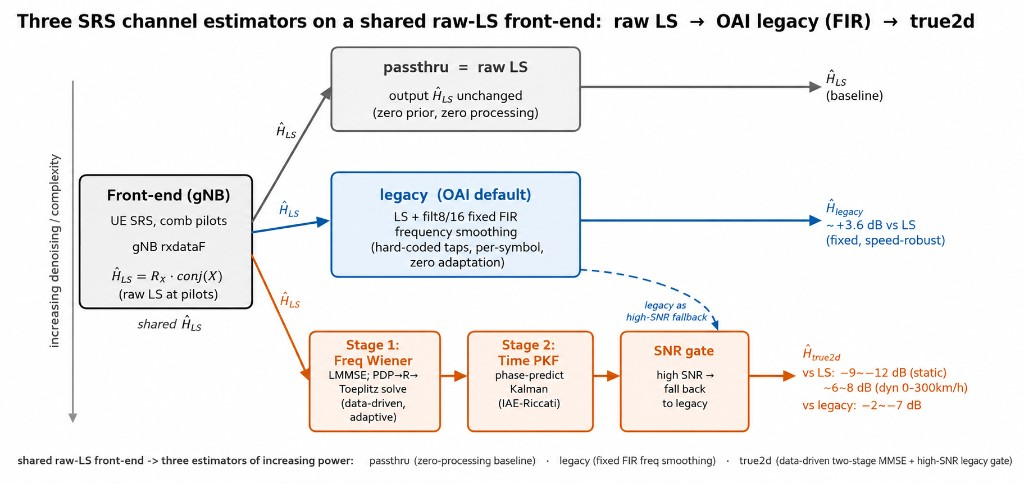
\includegraphics[width=0.96\textwidth]{figs/true2d_oai_architecture.png}
\end{center}
\vspace{-1mm}
{\footnotesize \LS\ = zero-processing baseline \;$\cdot$\; \LEG\ = LS + fixed filt8/16 FIR (OAI default) \;$\cdot$\; \TT\ = data-driven 2-stage MMSE + high-SNR legacy gate.}
\end{frame}

% ---------- Testbed ----------
\begin{frame}{3.\ Native testbed \& methodology}
\begin{itemize}
  \item \textbf{native rfsimulator + channelmod} (no proxy): direct noise control, channel truth = rfsim \texttt{channelDesc}, reproducible (fixed seed).
  \item \textbf{Ground-truth pipeline}: dump rfsim CIR taps + absolute timestamp $\to$ 2048-FFT $\to$ NMSE vs.\ SRS estimate (STO-aligned).
  \item \textbf{CDL dynamic replay}: 3GPP CDL-A..E rays $\to$ per-slot sample-spaced CIR (Doppler from angles) replayed into the uplink.
  \item \textbf{Validity gate}: STO-aligned complex coherence $\geq 0.5$; per point rep$=3$ median; per-launch 5GC restart (avoids NAS degradation).
\end{itemize}
\vspace{1mm}
{\footnotesize Correctness: offline vs.\ oracle $-28\!\sim\!-30$\,dB; C vs.\ golden bit-exact ($\leq 1$ LSB); SRS-vs-GT coherence $0.98\!\sim\!1.0$.}
\end{frame}

% ---------- Core three-way ----------
\begin{frame}{4.\ Core result: three-way NMSE (static + dynamic)}
\begin{center}
  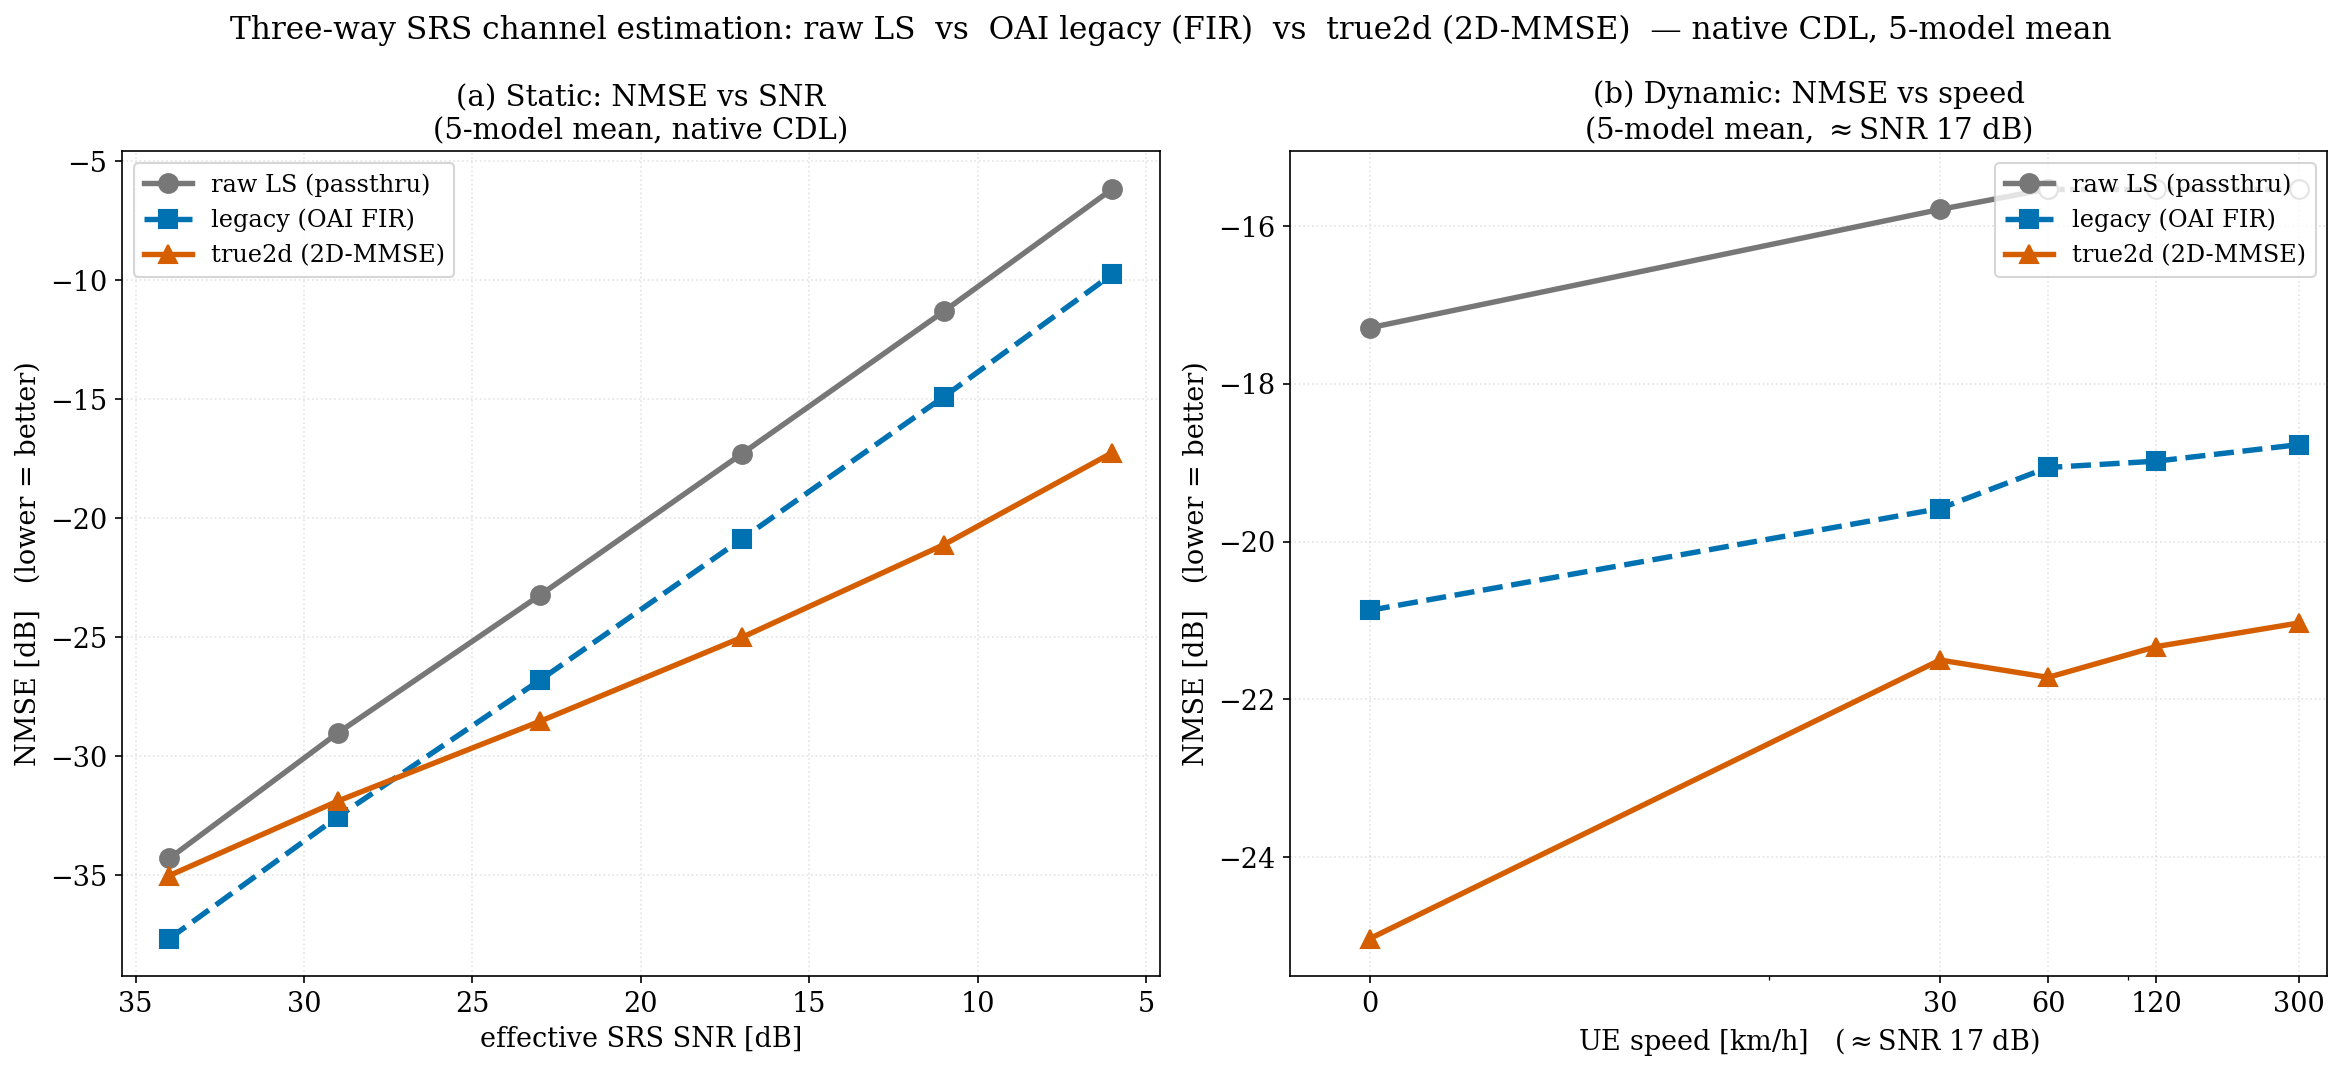
\includegraphics[width=0.97\textwidth]{figs/native_cdl_threeway_static_dynamic.png}
\end{center}
\vspace{-1mm}
{\footnotesize (a) Static vs.\ SNR: \TT\ best at mid/low SNR; \LEG\ slightly better at very high SNR (crossover $\approx$27\,dB).\quad
(b) Dynamic vs.\ speed: \TT\ lowest NMSE at all speeds.}
\end{frame}

% ---------- Static bars ----------
\begin{frame}{5.\ Static, cross-model ($\approx$SNR 11 dB)}
\begin{center}
  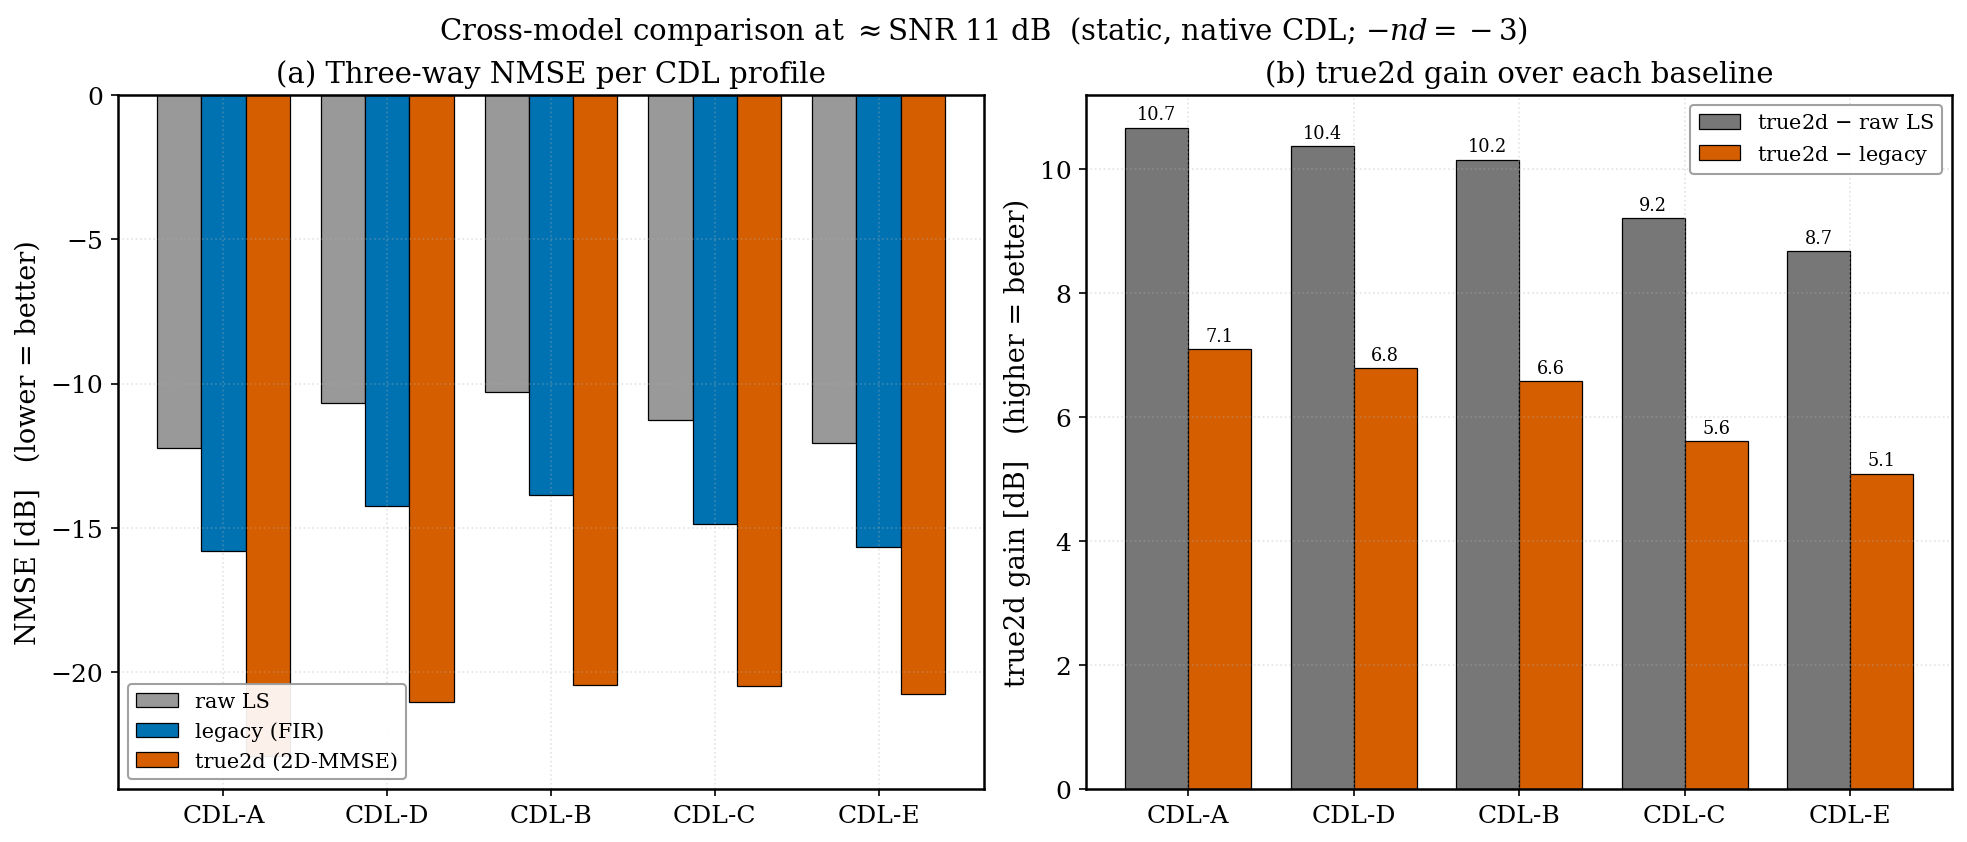
\includegraphics[width=0.92\textwidth]{figs/native_cdl_nd_minus3_bars.png}
\end{center}
\vspace{-1mm}
{\footnotesize \TT\ over \LS: \textbf{8.7--10.7\,dB}; over \LEG: \textbf{5.1--7.1\,dB}. Gain decreases with delay spread (A short $\to$ E long) — physically consistent (less freq correlation to exploit).}
\end{frame}

% ---------- Crossover + gate ----------
\begin{frame}{6.\ High-SNR crossover \& legacy gate}
\begin{columns}[T]
  \begin{column}{0.72\textwidth}
    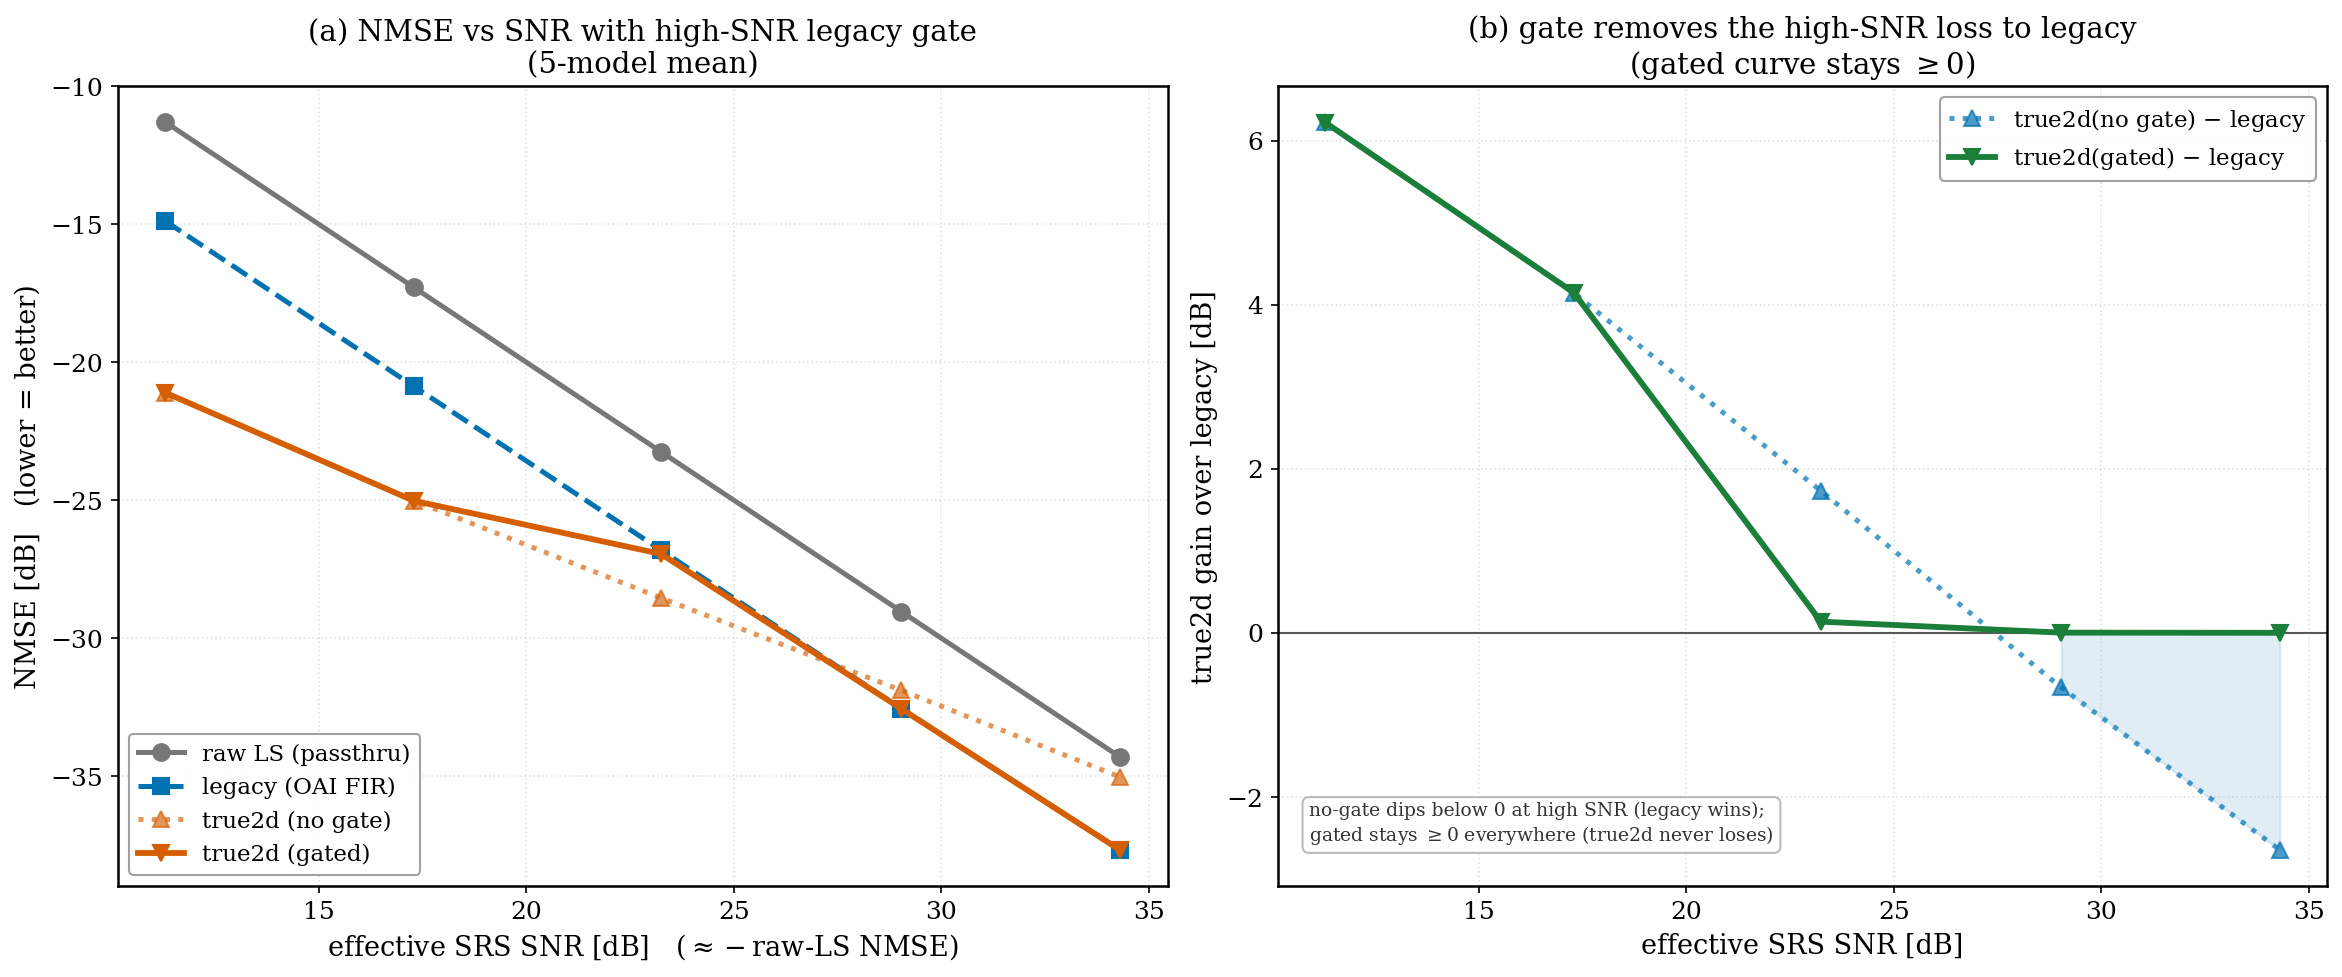
\includegraphics[width=\textwidth]{figs/native_cdl_3way.png}
  \end{column}
  \begin{column}{0.26\textwidth}
    \scriptsize
    At high SNR \LEG\ (near-lossless FIR) beats \TT\ (MMSE over-filters a near-perfect signal).\\[2mm]
    \textbf{SNR gate}: per-link, at high SNR blend \TT\ output back to the (free) \LEG\ estimate.\\[2mm]
    Result: \TT\ \textbf{never loses} to \LEG\ across all SNR, low-SNR wins kept.
  \end{column}
\end{columns}
\end{frame}

% ---------- Dynamic vs LS ----------
\begin{frame}{7.\ Dynamic: \TT\ vs.\ raw LS (0--60 km/h)}
\begin{center}
  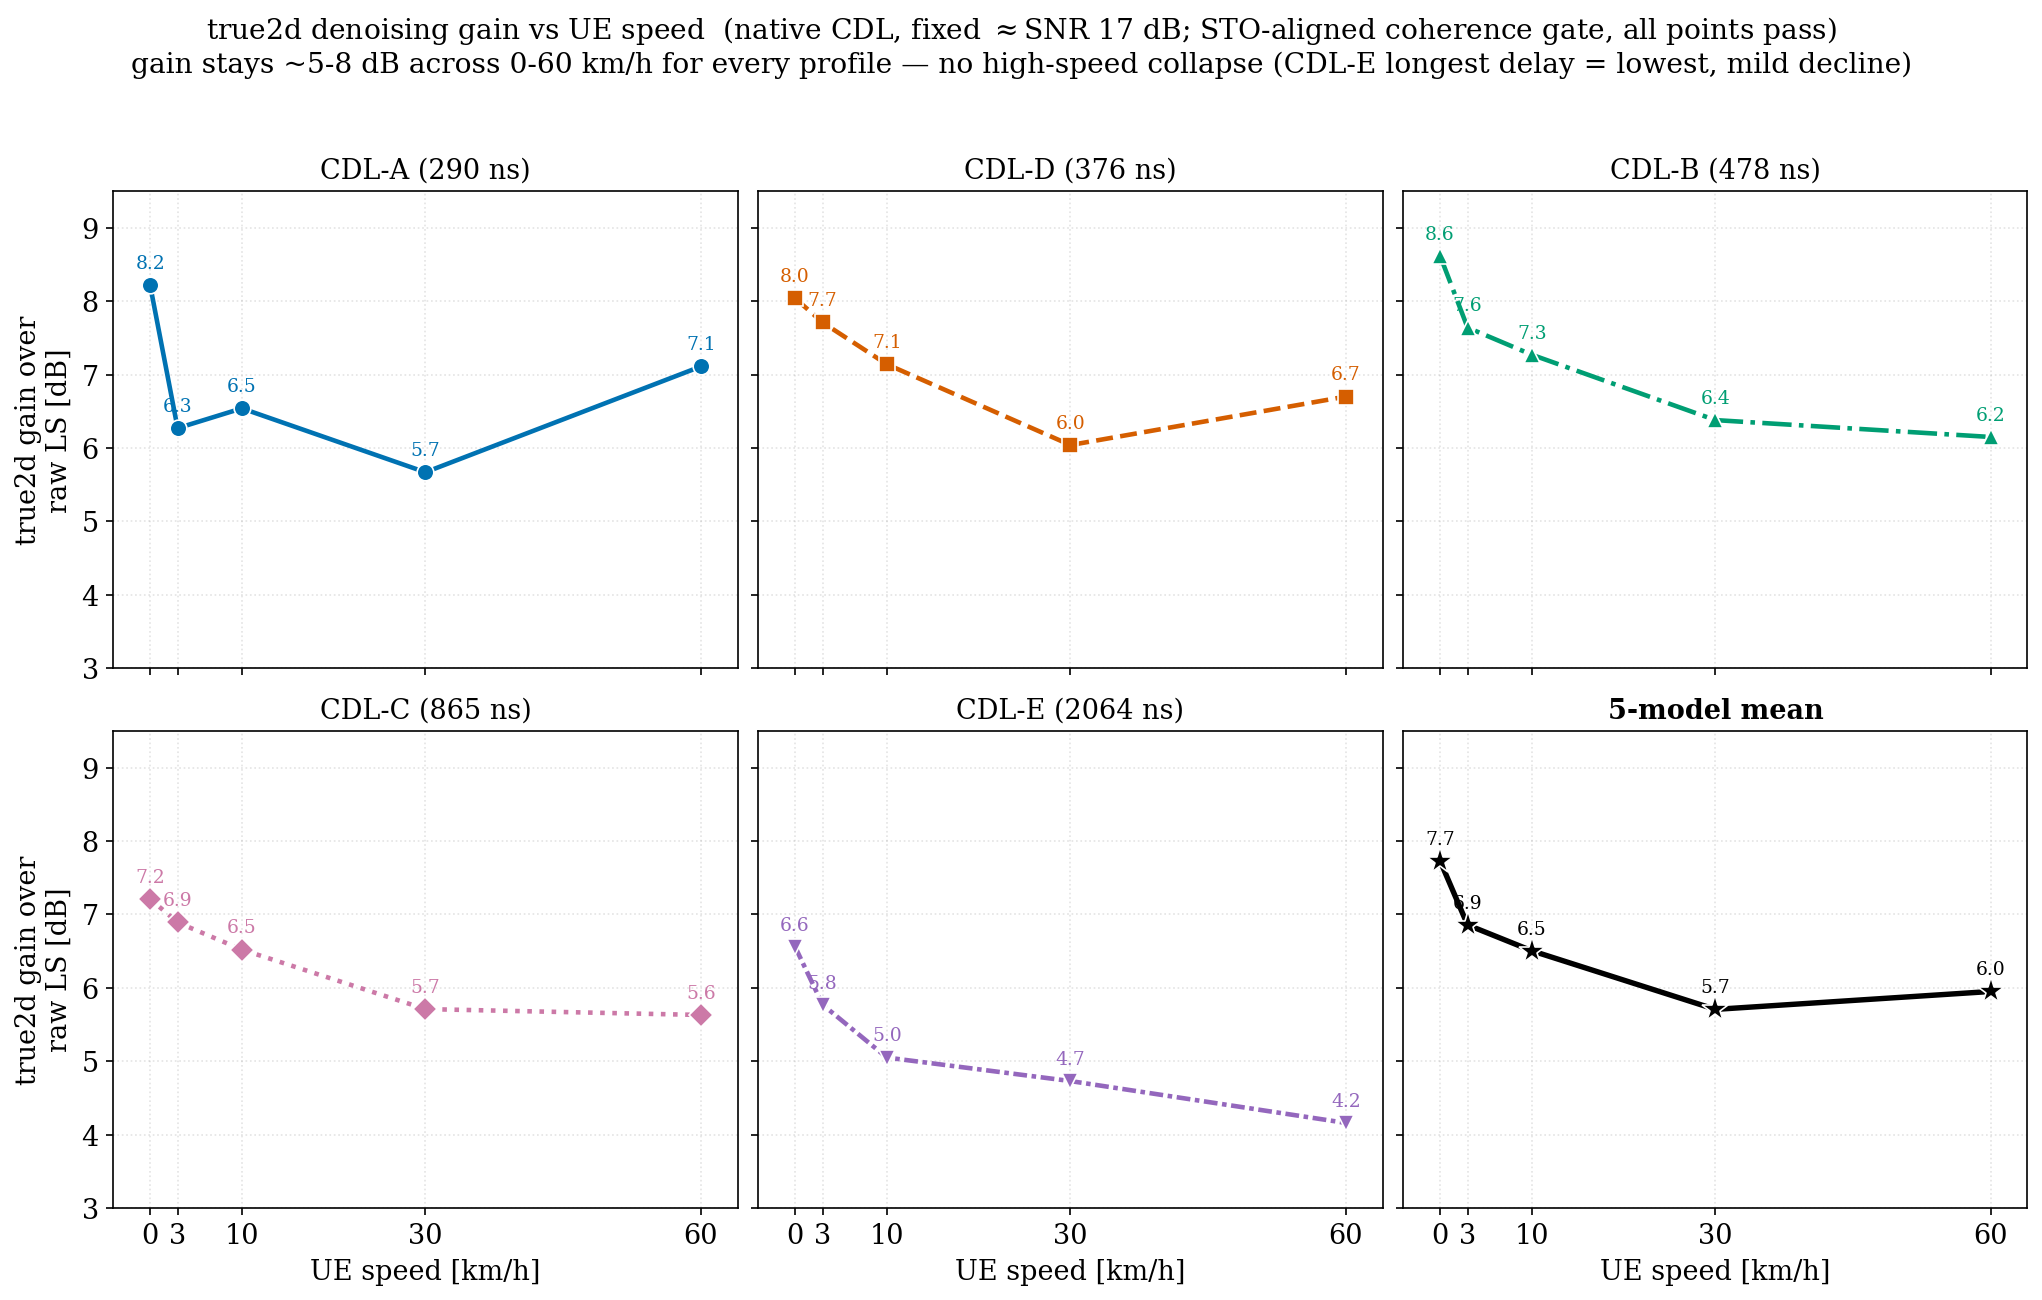
\includegraphics[height=0.60\textheight]{figs/native_cdl_gain_vs_speed.png}
\end{center}
\vspace{-1mm}
{\footnotesize Gain $\approx$\,6--8\,dB across 0--60 km/h, only $\sim$1--2\,dB drop static$\to$moving, then flat. Frequency-stage Wiener (per-frame, speed-independent) dominates.}
\end{frame}

% ---------- Dynamic vs legacy ----------
\begin{frame}{8.\ Dynamic: \TT\ vs.\ legacy, up to 300 km/h}
\begin{center}
  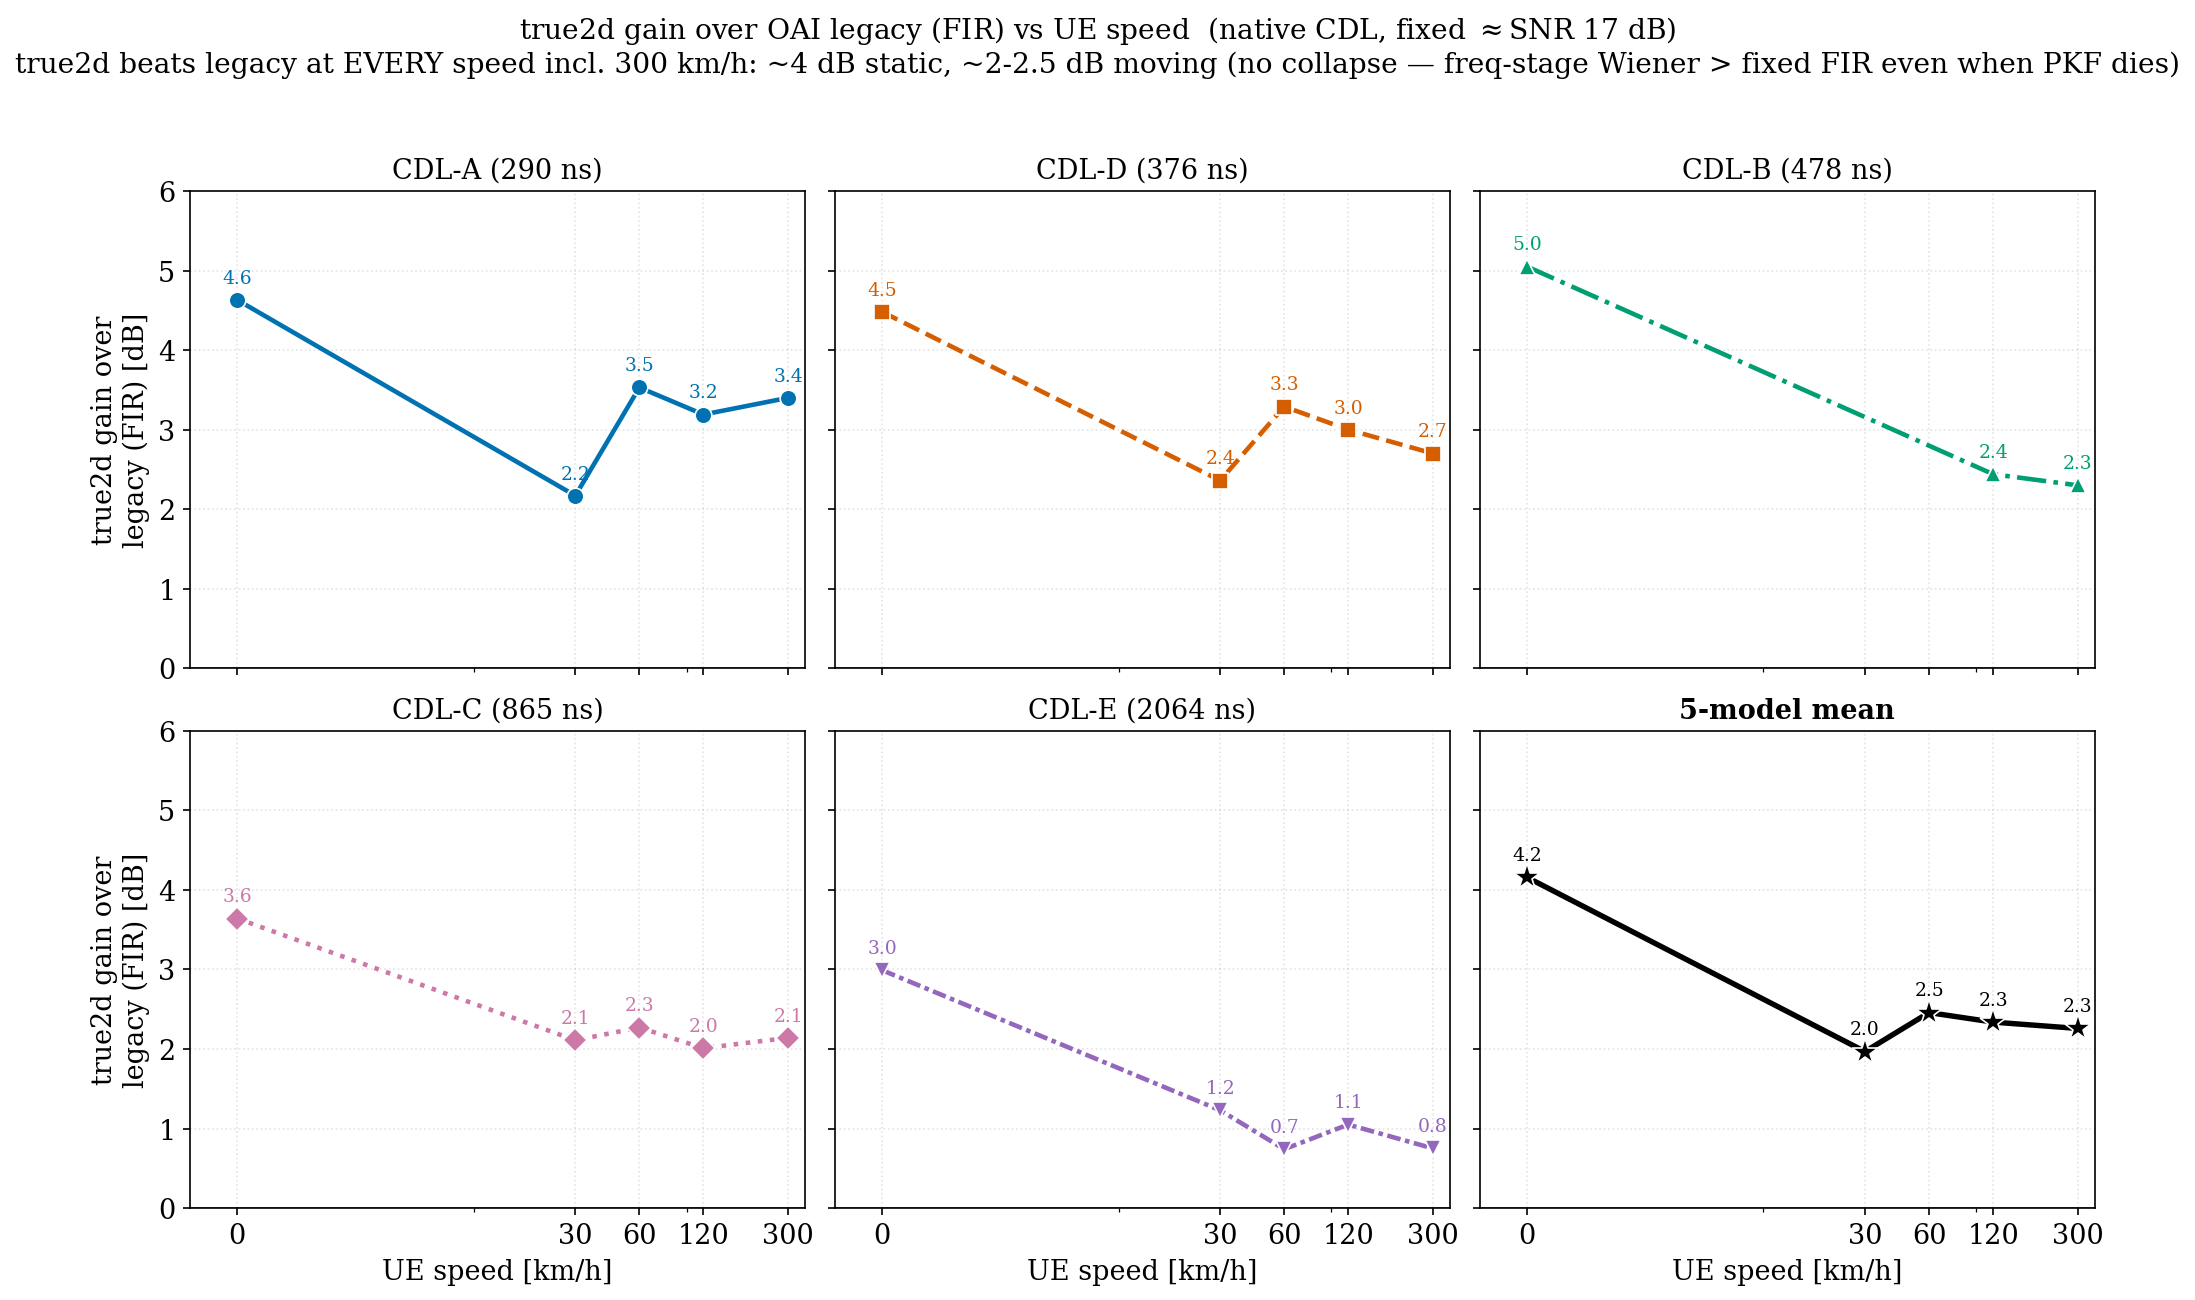
\includegraphics[height=0.60\textheight]{figs/native_cdl_gain_vs_speed_legacy.png}
\end{center}
\vspace{-1mm}
{\footnotesize \TT\ beats \LEG\ at \emph{every} speed incl.\ 300 km/h ($\sim$2--3.4\,dB). PKF dies at high Doppler but the freq-stage still $>$ fixed FIR $\to$ graceful degradation (IAE-Riccati).}
\end{frame}

% ---------- Summary ----------
\begin{frame}{9.\ Summary \& outlook}
\textbf{true2d gain (native CDL; min--max over CDL-A..E):}
\begin{center}\small
\begin{tabular}{lcc}
\toprule
 & vs.\ raw LS & vs.\ OAI legacy \\
\midrule
Static (mid--low SNR, $\approx$6--11 dB) & \textbf{up to 12} dB & \textbf{up to 7.5} dB \\
Dynamic 0--300 km/h ($\approx$SNR 17 dB) & $4.2\!-\!8.6$ dB & $0.7\!-\!5.1$ dB \\
\bottomrule
\end{tabular}
\end{center}
{\scriptsize Ranges = min--max across the 5 CDL profiles (and speeds, dynamic). Ceiling = short-delay (CDL-A/B/D); floor = CDL-E (2064 ns long delay). Values are where both estimators work normally (coh $\geq 0.5$).}
\vspace{2mm}
\begin{itemize}
  \item \textbf{Speed-robust}, no high-speed collapse; high-SNR gate $\Rightarrow$ never worse than legacy.
  \item Sweet spot = mid/low SNR, any speed; weakest at long delay (CDL-E) / very high SNR.
  \item \textbf{Next}: test true2d on the lab's current Gwanghwamun-area channel scenario to validate the gain under a realistic urban deployment profile.
\end{itemize}
\end{frame}

\end{document}
